\documentclass[12pt,letterpaper,boxed]{hmcpset}
\usepackage[margin=1in,headheight=14pt]{geometry}
\usepackage{amsfonts, amsmath, amssymb, enumerate, fancyhdr, gensymb, lastpage, mathtools, parskip, graphicx}
\usepackage{xcolor, tikz-cd}
\newcommand{\wg}[1]{\textcolor{violet}{#1}}
\newcommand{\OO}{\mathcal O}
\newcommand{\Q}{\mathbb Q}
\newcommand{\R}{\mathbb R}
\newcommand{\C}{\mathcal C}
\newcommand{\Z}{\mathbb Z}
\newcommand{\abs}[1]{\left|#1\right|}
\newcommand{\im}{\text{im }}
\newcommand{\tih}{\tilde h}
\newcommand{\inv}{^{-1}}
\newcommand{\normal}{\unlhd} %% one can also use \trianglelelefteq
\newcommand{\anglee}[1]{\langle #1 \rangle}
\usepackage[shortlabels]{enumitem}

% Numbering macros
\pagestyle{fancy}
\lhead{Will Gilroy}
\chead{Algs Homework \#}
\rhead{03 November 2021}
\lfoot{}
\cfoot{}
\rfoot{Page\ \thepage\ of\ \pageref{LastPage}}

\linespread{1.5}

\newcommand\blankpage{
    \thispagestyle{empty}
    \addtocounter{page}{-1}
    \newpage}
\renewcommand\footrulewidth{0.4pt}

\begin{document}

\problemlist{Algorithms HW } 

%------------------------- Problem 1 -----------------------

\begin{problem}
	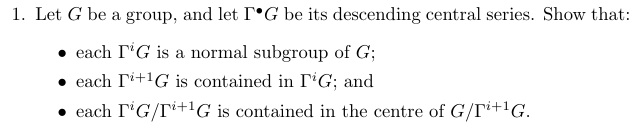
\includegraphics[scale=0.8]{1.png}
	\hfill
\end{problem}

\begin{solution}
\begin{itemize}
\item 
We show that $\Gamma^iG \normal G$ by induction on $i$. Since
$\Gamma^1 G = G$ our base case is $i=2$. Recall that $\gamma^2 G$ is
generated by commutators $[g,h]$ where $g, h \in G$. Now let $k \in G$
and consider 
\begin{align*}
	k [g,h] k\inv = k g h g\inv h\inv k\inv
	= (kgk\inv)(k h k\inv) (k g\inv k\inv) (k h\inv k\inv)
	= [k g k\inv, k h k\inv] \in \Gamma^2 G.
\end{align*}
And so, $\Gamma^2 G \normal G$ by definition.

Now suppose $\Gamma^i G \normal G$ and consider $\Gamma^{i+1} G$,
which is generated by elements $[g,h]$ where now $g \in G$ and $h \in
\Gamma^i G$. Let $k \in G$ and notice that, since $\Gamma^i G$ is
normal by the induction hypothesis, 
we have $k h k\inv \in \Gamma^iG$. Thus the above calculation
gives that $k[g,h]k \inv = [k g k\inv, k h k\inv] \in \Gamma^{i+1}G$.
Thus, each $\Gamma^i G \normal G$ by induction.

\item 
We show that $\Gamma^{i+1} G \subseteq \Gamma^i G$. Let $[g,h]$ be a
generator of $\Gamma^{i+1}G$ so that $g \in G$ and $h \in
\Gamma^{i}G$. 
Above we showed that $\Gamma^i G \normal G$ and so $ghg\inv \in
\Gamma^i G$. Moreover, $h \in \Gamma^i G$ implies $h\inv \in \Gamma^i
G$ since $\Gamma^i G$ is a group. Thus \[
	[g,h] = ghg\inv h\inv = (g h g\inv) h \in \Gamma^i G. 
\]
Then, since each generator of $\Gamma^{i+1} G$ is contained in
$\Gamma^i G$, we have $\Gamma^{i+1} G \subseteq \Gamma^{i}G$. 

\item \wg{todo}
\end{itemize}

\end{solution}

\newpage

%------------------------- Problem 2 -----------------------

\begin{problem}
	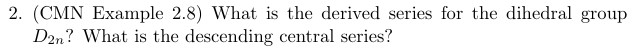
\includegraphics[scale=0.8]{2.png}
	\hfill
\end{problem}

\begin{solution}
I'm sorry I'm going to use $D_n$ to denote the dihedral group which
has $2n$ elements. Recall the presentation \[
	D_n = \langle 
		r,s : r^n = s^2 = e \quad rs = sr\inv 
	\rangle
\]

First note that $D_1$ and $D_2$ are abelian. 
We have $D_1 = \{ e, s \}$ a single non-trivial element, and so is
trivially abelian. Meanwhile $D_2 = \{ e, s, r, rs \}$, the relation 
$rs = sr\inv$ becomes $rs = sr$, i.e. $[r,s] = e$. Likewise we have 
$[r,rs] = r(rs)r(rs)\inv = r^2 (rs)(rs)\inv = e$ and 
$[s, rs] = s (rs) s (rs)\inv = s^2 (rs) (rs)\inv = e$\footnote{
I later realized that computing $[g,h]$ is enough to determine
$[h,g]$. In particular if $[g,h] = x$ for some $x \in G$ then we have
$ghg\inv h\inv = x \implies x\inv = h g h\inv g\inv = [h,g]$. Alas,
there is some redundent calculation above.
}. Hence, $D_2$ is
also abelian. \wg{Question: was it sufficient to show that $r,s$
commute to show that $D_n$ is abelian? And generally speaking, if a
group is generated by $n$ elements $g_1, \cdots g_n$ which all
commute, is that sufficient to show that the group is abelian?}
\wg{(later), okay I have convinced myself. I think in general 
showing that all the generators of a finite group commute with each other is
enough to show that every commutator of a group is trivial.}

It follows that the
derived subgroup $G' = \Gamma^2 G$ is trivial for $G = D_1$ or $G =
D_2$.
Moreover, since $\Gamma^3 G$ is generated by $[g, e] = g e
g\inv e = e$ for each $g \in G$, it follows that $\Gamma^i G$ is
trivial for each $i > 1$ for both of these groups.

Now suppose $n \geq 3$ is odd. We show first that $\Gamma^2 G =
\langle r \rangle$ by computing all the commutators. Recall that
$\Gamma^2 G = G'$ is the subgroup generated by all commutators $[g,h]$
where $g \in G$ and $h \in \Gamma^1 G = G$. We need to compute the
following commutators: $[r^k,s], [r,r^ks], [s,r^ks]$ where $k = 1,
\cdots, n-1$. First recall the relation $rs = s r\inv$ and then
consider the following \[
	[r^k, s] = r^k s r^{-k} s = r^k r^{-k} s^2 = r^{-2k} \neq e
\]
where the last equality follows from the fact that $n$ is odd.
In particular $k=1$ shows that $r^2 \in \Gamma^2 G$. 
Very similar calculations give the following
\begin{align*}
	[r, r^ks] &= r (r^k s) r\inv (s r^{-k}) = r^2 \neq e \\
	[s, r^ks] &= s(r^k s) s (s r^{-k}) = r^{-2k} \neq e
\end{align*}
Then, since we have already shown that $r^2 \in \Gamma^2 G$ we have
that $\Gamma^2 G = \langle r^2 \rangle$. The situation is even better
than this because for $n \geq 3$ odd we have $\langle r^2 \rangle =
\langle r \rangle$. We have $r^2 = r \cdot r \in \langle x \rangle$.
Moreover, consider there are $n$ distinct powers of $r$ in $\langle
r^2 \rangle$, we have \[
\langle r^2 \rangle = \{r^2, r^4, \cdots, r^{n + 1} = r, r^{n+3}, \cdots,
r^{2n-2}, e\},
\]
since, again, $n$ is odd. That is, we have $r \in \langle r^2 \rangle$
and so indeed we have \[
	\Gamma^2 G = \langle r^2 \rangle = \langle r \rangle.
\]

Next we show that when $\Gamma^{i-1} G = \langle r \rangle$  then we
must have $\Gamma^i G = \anglee r$ for $i = 3, 4, \dots$ 
Recall that $\Gamma^i G$ is generated by $[g,h]$ where $g \in G$ and
$h \in \Gamma^{i-1}G$. Since $\Gamma^{i-1}G$ is only generated by a
single element we only need to compute the following:
\begin{align*}
	[r^k, r] &= e\\
	[s, r] &= r^{-2}\\
	[r^ks, r] &= r^{-2},
\end{align*}
following similar calculations to above. That is $\Gamma^i G = \anglee
{r^2}$ and we still have $\anglee{r^2} = \anglee r$, since this was a
property of the group $D_n$ for $n \geq 3$ odd.
That is, we have shown $\Gamma^i G = \anglee r$ for $i \geq 2$. 

Now we consider the case when $n \geq 4$ is even. First notice that we
can split this case into two further cases --- either $n = 2^k$ for
some $k$ or $n = 2^km$ for some $k$ and some $m \geq 3$ odd. If $n$ is
not a power of $2$ then its prime factor decomposition is $2^k m$
where $m$ is the product of all of its odd prime factors.

Now first consider the case where $n = 2^km$. Our above calculation
shows that $\Gamma^{2}D_{2^km} = \anglee{r^2}$ but now $\anglee{r^2}
\neq \anglee r$ since $r^2$ has even order. In particular
$\anglee{r^2} = \{r^2, r^4, \cdots, r^{2\cdot(2^{k-1}m)} = e\}$. 
Now we compute $\Gamma^3 G$ via direct computation of the generators
$[g,h]$ where $g \in G$ and $h \in \Gamma^2G = \anglee{r^2}$.
Following the now usual strategy, we have 
\begin{align*}
	[r^k, r^2] &= e \\
	[s, r^2] &= sr^2 s r^{-2} = r^{-4} \\
	[r^ks, r^2] &= r^{-4}.
\end{align*}
That is, $\Gamma^3 G = \anglee{r^4}$. Essentially the same calculation
will give $\Gamma^i G = \anglee{r^{2^{(i-1)}}}$ for $2 \leq i$.

\end{solution}

\newpage

%------------------------- Problem 3 -----------------------

\begin{problem}[3]
	\hfill
\end{problem}
\begin{solution}
\end{solution}

\newpage

%------------------------- Problem 4 -----------------------

\begin{problem}
	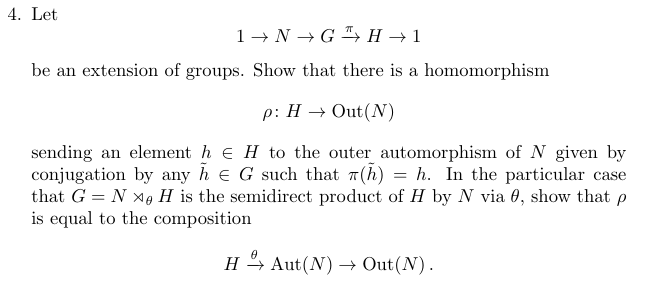
\includegraphics[scale=0.8]{4.png}
	\hfill
\end{problem}

\begin{solution}
Firstly, we will show that $\rho$ is a well defined map $H \to
Out(N)$. Let $h \in H$ and $\tih_1, \tih_2 \in G$ such that $\pi(\tih_1)
= \pi(\tih_2) = h$. We have 
$\rho(\tih_1) = f := (n \mapsto \tih_1 n \tih_1\inv)$ and
$\rho(\tih_2) = g := (n \mapsto \tih_2 n \tih_2\inv)$. 
Note that these are indeed automorphisms of $N$, as in the previous
homework we showed that conjugation by a fixed element is an
automorphism.
If we show that $\rho(\tih_1)$ and $\rho(\tih_2)$ lie in the same
coset of $Inn(N)$ then $\rho$ is well-defined. (Note: I believe this
map is not well defined as a map $H \to Aut(N)$). 

Recall that two elements $g,h$ of a group lie in the same coset of a normal
subgroup $N$ if $g\inv h \in N$. For our automorphisms $f,g$ we have
$g\inv = (n \mapsto \tih_2\inv n \tih_2)$. And so we have 
$(g\inv \circ f)(n) = \tih_2\inv \tih_1 n \tih_1\inv \tih_2$. Recall
that $N \normal G$ and so is closed under conjugation by definition.
In particular then $\tih_1 n \tih_1\inv \in N$ and $\tih_2\inv(\tih_1
n \tih_1 \inv) \tih_2 \in N$ since $\tih_1, \tih_2 \in G$. 
Thus $f,g$ have the same image in $Out(N)$ and so $\rho$ is well
defined with respect to the choice of $\tih$. 

Next we show that $\rho$ is a group homomorphism. Let $h_1, h_2 \in H$
and $\tih_1, \tih_2 \in G$ such that $\pi(\tih_1) = h_1$ and
$\pi(\tih_2) = h_2$. Moreover, since $\pi$ is a group homomorphism we
have $\pi(\tih_1\tih_2) = \tih_1 \tih_2$. Following a similar,
calculation to last week's homework, consider the following

\begin{align*}
	\rho(h_1h_2) &= \gamma_{\tih_1\tih_2} \\
		&= (n \mapsto \tih_1\tih_2 n (\tih_1\tih_2)\inv) \\
		&= (n \mapsto \tih_1 \tih_2 n \tih_2\inv \tih_1\inv) \\
		&= \gamma_{\tih_1} \circ \gamma_{\tih_2} \\
		&= \rho(h_1)\rho(h_2).
\end{align*}
Thus, the given $\rho$ is indeed a group homomorphism.

Now suppose $G = N \rtimes_\theta H$. We can state more precisely the
outer automorphism given by $\rho$. Let $h \in H$ and then all lifts
are of the form $\tih = (m, h)$ for some $m \in N$. Then, being
explicit about the details of the semidirect product, our map
$\rho(h) : \iota(N) \to \iota(N)$ acts as follows 
\begin{align*}
	\rho_h(n) &= (m, h) \cdot_\theta (n, e_H) \cdot_\theta (m, h)\inv \\
		&= (m,h) (n, e_H) (\theta_{h\inv}(m\inv), h\inv) \\
		&= (m \theta_h(n), h) (\theta_{h\inv}(m\inv), h\inv) \\
		&= (m \theta_h(n) (\theta_h \circ \theta_{h\inv}(m\inv), h h\inv) \\
		&= (m \theta_h(n) m\inv, e_H).
\end{align*}
Which induces the automorphism $f = (n \mapsto m\theta_h(n)m\inv) : N \to
N$. Note that $(\theta_{h} \theta_{h\inv}) = id_H$ since $\theta$ is a
group homomorphism $H \to Aut(N)$. 

We show that this is the same as the composition $H \to Aut(N) \to
Out(N)$. We have $h \mapsto \theta_h \mapsto \overline{\theta_h}$. 
Notice now that $\theta_h$ and $f$ are lie in the same coset of
$Inn(N)$. In particular \[
	\overline{\theta_h} = \overline{\gamma_m \theta_h} = \overline{f}
\]
since $\gamma_m = (n \mapsto m n m\inv)$ is one of the inner
automorphisms of $N$.
Hence, in the case where $G = N \rtimes_\theta H$ we have $\rho$ and
$H \to Aut(N) \to Out(N)$ give the same map.

One interpretation of this is that, whilst $\rho$ is a well defined
map $H \to Out(N)$, it is not a well defined map $H \to Aut(N)$.
However, in the case where $G$ is a semidirect product of $N$ and $H$
via $\theta$,
we have a preferred lift $h \mapsto (e_N, h) \in G$, 
and in fact there is a well defined map $H \to Aut(N)$, namely
$\theta$, whose projection gives the same map as $\rho$. 


\end{solution}

\newpage
%------------------------- Problem 5 -----------------------

\begin{problem}
    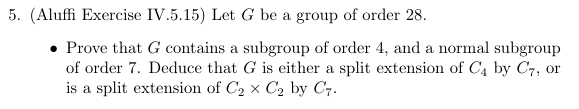
\includegraphics[scale=0.8]{5-1.png}
	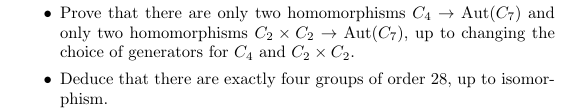
\includegraphics[scale=0.8]{5-2.png}
	\hfill
\end{problem}

\begin{solution}
\begin{itemize}
\item Sylow's theorem I gives us that there exists a subgroup of order
$7$ in $G$, since $\abs{H} = 7^1 \cdot 4$ and $7 \not \vert 4$. 
Alternatively, Cauchy's theorem gives us that there exists an element
$g \in G$ with $\abs{g} = 7$, hence we have $\abs{\langle g \rangle}
\leq G$. Moreover, Sylow III gives us that there's only a single Sylow
$7$ group. Consider, if $n_7$ is the number of Sylow $7$ groups in
$G$ then Sylow III gives us that $n_7 \equiv 1 \mod 7$ and $n_7 \vert
4$. The only integer solving both these conditions is $n_p = 1$. 
Likewise if we write $\abs G = 28 = 2^2 \cdot 7$ and notice $2
\not\vert 7$ then Sylow I gives us that there exists a subgroup of
order $2^2 = 4$.

Next we argue that $N$ is normal. If $g \in G$ then recall $\gamma_g =
(\ell \mapsto g\ell g\inv) \in Aut(G)$. Therefore $\abs{\gamma_g(N)} =
\abs{N}$. However, there's a unique subgroup of order $7$ in $G$ and
so the image $\gamma_g(N) = N$ for all $g \in G$. That is, $N$ is
closed under conjugation by elements in $G$ and so $N$ is normal by
definition. We have shown that $G$ has a normal subgroup of order $7$
and in fact we have found that $N \cong C_7$.


\item Recall \wg{or perhaps I shall prove} that $Aut(N) = Aut(C_7)
\cong C_6$. Consider $C_4$, once we have specified where a generator
$\sigma \in C_4$ is mapped to in $C_6$ then we have determined the
homomorphism $C_4 \to C_6$.
Since $\abs \sigma = 4$ we must have $\abs{\theta(\sigma)} = 4$ or
$\abs{\theta(\sigma)} = 2$, for $\theta$ non-trivial,
 since a homomorphism must map an element
to an element whose order divides the original order.
Notice that there's only a single element of order $2$ in $C_6$. And
so there's one trivial map and one non-trivial map $\overline \theta: C_4
\to N$.
Since $\overline\theta(\sigma)$ has order two we can deduce that it is the
automorphism which sends each element of $C_7$ to its inverse. That is 
$\overline\theta(\sigma) = (n \mapsto 7 - n)$. And, of course, the
trivial map $\theta_{\text{triv}}(\sigma) = (n \mapsto 0)$ for each
$\sigma \in C_4$. 

We use similar reasoning to determine the maps $\theta: C_2 \times C_2
\to Aut(N) \cong C_6$. One generating set of $C_2 \times C_2$ is
$\{(0,1), (1,0)\}$ and again, once we determine where these elements
are mapped to by $\theta$ we have determine the entire homomorphism
$\theta: C_2 \times C_2 \to C_6$. Now each generating element has
order two, and so any non-trivial $\theta$ maps both the generating
elements to the unique element of order $2$ in $C_6$. 
And so, again, we have one trivial map $\theta_{\text{triv}}: C_2
\times C_2 \to C_6$ and one non-trivial map $\tilde \theta: C_2 \times
C_2 \to C_6$. The automorphisms $\tilde \theta((0,1)) =
\tilde\theta(1,0)$ are both the same as the one described above ---
$(n \mapsto 7 - n \equiv -n)$.

\item Determining all the possible semi-direct products $C_7 \rtimes
H$ with $H = C_4$ or $H = C_2 \times C_2$ will tell us the possible
group laws on $G$. Notice that $N \cap H = \{e \}$ for $H = C_4$ or
$C_2 \times C_2$, this follows since every element of $N \cong C_7$ is
the identity or is order $7$, meanwhile there are no elements of order
$7$ in either $C_4$ or $C_2 \times C_2$. 
\wg{We also need to show that $NH = G$}. 
Then it follows that $G \cong N \rtimes_\theta H$ for $H = C_4$ or $H
= C_2 \times C_2$ and one of the $\theta$ described above.

With all possible homomorphisms $H \to Aut(N)$ described above,
we can determine all the semi-direct products $N \rtimes H$.
First suppose $H = C_4$ and $\theta : C_4 \to C_6$ the trivial map.
That is $\theta(h) = (n \mapsto n)$ for each $h \in H$. We have the
following group product for $N \rtimes_\theta H$:
\begin{align*}
	(n_1, h_1) \cdot_\theta (n_2, h_2) 
		&= (n_1 \theta_{h_1}(n_2), h_1 h_2) \\
		&= (n_1 n_2, h_1 h_2).
\end{align*}
That is, then $N \rtimes_\theta H$ is isomorphic to $C_7 \times C_4
\cong G$.
The same calculation will give us that when $H = C_2 \times C_2$ and
$\theta : C_2 \times C_2 \to Aut(N)$ is the trivial map, we also have
$G \cong C_7 \times C_2 \times C_2$. 

Now we determine the products given by the non-trivial $H \to Aut(N)$.


\end{itemize}
\end{solution}

\newpage
%------------------------- Problem 4 -----------------------

\begin{problem}[4]
	\hfill
\end{problem}

\begin{solution}
\end{solution}

\newpage

%------------------------- Problem 4 -----------------------

\begin{problem}[4]
	\hfill
\end{problem}

\begin{solution}
\end{solution}

\newpage

%------------------------- Problem 4 -----------------------

\begin{problem}[4]
	\hfill
\end{problem}

\begin{solution}
\end{solution}

\newpage



\end{document}
